\chapter{Results}
\label{sec:results}

In the current chapter, results of GAT-Denoiser are presented.
Further, some interesting findings are illustrated and GAT-Denoiser
is compared to U-Net and BM3D\cite{bm3d}.


\section{Dataset}
GAT-Denoiser is tested on lodopab-ct dataset \cite{lodopab-dataset}, which is a 
benchmark dataset for low-dose ct reconstruction methods and therefore well suited for our domain.

The dataset consists of 35820 train images and 3553 test images.
All these images are having resolution 64.

\begin{figure}[H]
  \centering
  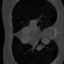
\includegraphics[width=0.2\textwidth]{ct_im_0.png}
  
\includegraphics[width=0.2\textwidth]{ct_im_1.png}
  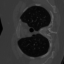
\includegraphics[width=0.2\textwidth]{ct_im_2.png}
  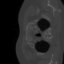
\includegraphics[width=0.2\textwidth]{ct_im_3.png}
  \caption{Some train images of lodopab-ct dataset.}
\end{figure}



\section{Training setup}
Training of GAT-Denoiser has been done on the HPC-cluster scicore of the University of Basel.
During training, up to 4 titanx GPUs with 12GB RAM have been used.


\section{Source code}
Source code of the project is available on github\footnote{https://github.com/cedricmendelin/master-thesis}.

\subsection{Python packages}
The following important python packages have benn 




Show most interesting results:
\begin{itemize}
  \item k-NN
  \item GAT Architecture
  \item L1 vs. L2
  \item Comparing with Bm3D (and/or non-local means).
\end{itemize}
